\documentclass{article}
\usepackage{amsmath}
\usepackage{amssymb}
\usepackage{setspace}
\usepackage{physics}
\usepackage{mathrsfs}
\newenvironment{nscenter}
{\parskip=0pt\par\nopagebreak\centering}
{\par\noindent\ignorespacesafterend}
\usepackage{graphicx}
\graphicspath{ {images/} }
\begin{document}
\begin{spacing}{1.5}
\section*{1 Four special matrices}
1. Toeplitz matrix

A Toeplitz matrix or diagonal-constant matrix, named after Otto Toeplitz, is a matrix in which each descending diagonal from left to right is constant. For instance:
\\\begin{center}
	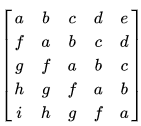
\includegraphics[width=0.2\textwidth]{Toeplitz_matrix1.png} \\ 
\end{center}
2. Circulant matrix

a circulant matrix is a special kind of Toeplitz matrix where each row vector is rotated one element to the right relative to the preceding row vector. For instance:
\\\begin{center}
	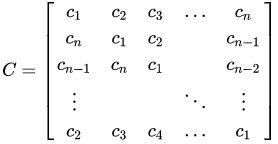
\includegraphics[width=0.35\textwidth]{circulant_matrix.png}
\end{center}

In numerical analysis, circulant matrices are important because they are diagonalized by a discrete Fourier transform, and hence linear equations that contain them may be quickly solved using a fast Fourier transform.
\\\\3. Change $T_{11}$ in Toeplitz matrix

Here we've a free variable in Toeplitz matrix $T$ at position $T_{11}$.
\\\\4. Change $T_{11}$ and $T_{nn}$ in Toeplitz matrix

Here we've two free variables in Toeplitz matrix $T$ at position $T_{11}$ and $T_{nn}$.


\section*{2 Differential eqns and Difference eqns}
Part 1. Notation of high order derivative

For n-th derivative, the notation is $\frac{d^ny}{dx^n}$ or $\frac{d^nf(x)}{dx^n}$. Sample of meaning of this notation: $\frac{d^2y}{dx^2}=\frac{d}{dx}(\frac{dy}{dx})$.
\\\\Part 2. First order difference

To calculate first order discrete derivative(difference) of $u(x)$, we have three choices: forward, backward and centered:

\hspace*{2cm}forward $\Delta_F$: $u'(x)\approx \frac{u(x+h)-u(x)}{h}$

\hspace*{2cm}backward $\Delta_B$: $u'x)\approx \frac{u(x)-u(x-h)}{h}$

\hspace*{2cm}centered($\frac{forward - backward}{2}$) $\Delta_C$: $u'(x)\approx \frac{u(x+h)-u(x-h)}{2h}$ 

We would like use centered difference for first order difference. The reason comes from the loss of accuracy:

First, recall Taylor series:
\begin{nscenter}
$f(x) = f(a)+{\frac {f'(a)}{1!}}(x-a)+{\frac {f''(a)}{2!}}(x-a)^{2}+{\frac {f'''(a)}{3!}}(x-a)^{3}+\cdots$
\end{nscenter}

Second, from Taylor series, we have:
\begin{nscenter}
$u(x+h)=u(x)+hu'(x) + \frac{h^2}{2!}u''(x) + \frac{h^3}{3!}u'''(x) + \cdots$
$u(x-h)=u(x)-hu'(x) + \frac{h^2}{2!}u''(x) - \frac{h^3}{3!}u'''(x) + \cdots$
\end{nscenter}

Finally, inserting $u(x+h)$, $u(x-h)$ in three kind of differences, $\Delta_F = \Delta_B \approx u'(x) + o(h)$, $\Delta_C\approx u'(x) + o(h^2)$.
\\\\Part 3. Second order difference

The best way to calculate second order discrete derivative(difference) is $u''(x) \approx \frac{-u(x+h) + 2u(x) -u(x-h)}{h^2}$, or $h$ with 1 such that $u''(x) \approx -u(x+1) + 2u(x)-u(x-1)$. You may wonder where this form comes from. This form is $\Delta_F\Delta_B(=\Delta_B\Delta_F)$, which is better than $\Delta_C \Delta_C$.

Having $\Delta(\Delta u(x)) = -u(x+1) + 2u(x)-u(x-1)$, we can write multi $\Delta(\Delta u(x))$ in matrix form. Here is a funny thing to see in the matrix form

$$
\Delta = 
\begin{bmatrix}
1 & 2 & -1 \\
  & 1 & 2 & -1 \\
  &   & 1 & 2 & -1
\end{bmatrix}
\begin{bmatrix}
u(i-2) \\
u(i-1) \\
u(i) \\
u(i+1) \\
u(i+2)
\end{bmatrix}
$$

Above is the second order difference of $u(x)$ at five points with gap 1. You can insert the five point with any function $g$. If the function is a linear/quadratic function, $\Delta$ is a vector with all element being 0/a constant! You can check this. The reason behind the funny thing is that $\Delta$ is second order discrete derivative. Also note that the matrix composed of 1, 2, -1 is a Toeplitz matrix.
\\\\ Part 3. Differential equations

For example, $-\frac{d^2u}{dx^2}=1$, $\frac{du}{dx}(0)=0$, $u(1)=0$. 

This is very easy to calculate.


\section*{3 Solving a Linear System}
Part 1. Four matrix decompositions

All these four decompositions are covered in 18.06 Linear Algebra.

Elimination: $A=LU$ and $A=LDU$

Orthogonalization: $A=QR$

Eigenvalues: $A=S\Lambda S^{-1}$

Singular values: $A=U\Sigma V^T$
\\Supplement:

For a matrix $A=BDB^T$, where $D$ is a diagonal matrix, $A$ is symmetric, since $A^T=BD^TB^T=BDB^T=A$. Then LDU decomposition on $A$, we get $A=LDL^T$.
\\\\Part 2.

More detail is needed.

For $AX=I$, we know $X=A^{-1}$. The deep insight is that columns of $A^{-1}$ are responses to $n$ impulses(columns of $I$).


\section*{4 Delta function day}
Part 1. Definition of Delta function

The Dirac delta can be loosely thought of as a function on the real line which is zero everywhere except at the origin, where it is infinite,
\begin{nscenter}
${\displaystyle \delta (x)={\begin{cases}+\infty ,&x=0\\0,&x\neq 0\end{cases}}}$
\end{nscenter}
and which is also constrained to satisfy the identity,
\begin{nscenter}
	${\displaystyle \int _{-\infty }^{\infty }\delta (x)\,dx=1}$
\end{nscenter}
\\\\Part 2. Delta function and differential eqns

For example, 
$$
\begin{cases}
-\frac{d^2u}{dx}=\delta(x-a), where \, 0 < a < 1 \qquad (1)\\
u(0)=0 \qquad (2)\\
u(1)=0 \qquad (3)
\end{cases}$$

To get the solution of $u(x)$, first let's see what equation (1) means. (1) tells us that $u(x)$ consists two lines, and there is a turning point, because only in this way can we get (1), for instance(not the solution for (1), (2), (3):)
\\\begin{center}
	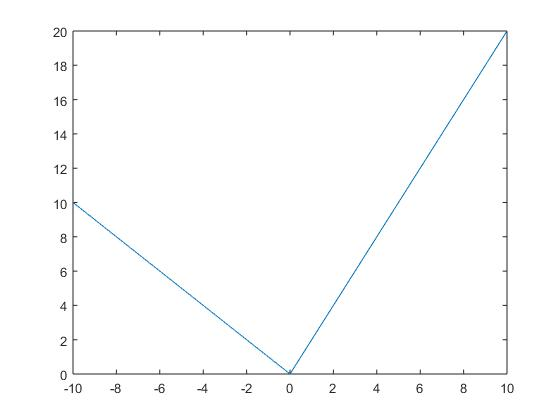
\includegraphics[width=0.4\textwidth]{piecewise_func.jpg} \\ 
\end{center}

But we have a better way to decompose the picture above as $u(x) = -R(x-a) + C + Dx$, where $R(x)$ is Ramp function. There are many equivalent definitions of Ramp function, here are two of them. 
\begin{nscenter}
	$R(x):={\begin{cases}x,&x\geq 0;\\0,&x<0\end{cases}}$ \qquad ${\displaystyle R(x):=\operatorname {max} (0, x)} $
\end{nscenter}

The convenience of $u(x) = -R(x-a) + C + Dx$ is that we can easily insert equations (2) and (3) to get $C$ and $D$.
\\\\Part 3. Boundary in differential eqns

We name equations (2) and (3) as boundaries in the differential eqns in part 2. Boundaries as $u(x)=a$ and $u'(x)=a$ are called fixed boundary and free boundary.

You can see that if we have at least one fixed boundaries, we can get only one solution. If the two boundaries are both free boundaries, we have numerous solutions.

\section*{5 \& 6 \& 7 Eigenvalues \& positive definite}
Covered in 18.06 Linear Algebra.


\section*{8 Springs and masses; the main framework}
Suppose, as below, here are $4$ springs and $3$ masses. The force comes from the $i$th spring is $w_i=c_ie_i$, where $c_i$ is the constant for spring $i$, $e_i$ is the elongation in spring $i$. And the displacement for the $i$th mass is $u_i$. 
\\\begin{nscenter}
	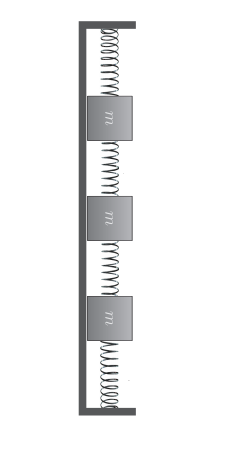
\includegraphics[width=0.2\textwidth]{four_springs_three_masses.png} \\ 
\end{nscenter}

It's easy to show $e_1 = u_1$, $e_2=u_2-u_1$, and so on. And $w_1 = c_1e_1$, $w_2=c_2e_2$, and so on. Write these equations in matrix form:
$$
\begin{bmatrix}
e_1 \\
e_2 \\
e_3 \\
e_4
\end{bmatrix}
=
\begin{bmatrix}
1  &   &  \\
-1 & 1 & \\
   & -1& 1\\
   &   & -1 
\end{bmatrix}
\begin{bmatrix}
u_1 \\
u_2 \\
u_3 \\
u_4 \\
\end{bmatrix}
$$

$$
\begin{bmatrix}
w_1 \\
w_2 \\
w_3 \\
w_4
\end{bmatrix}
=
\begin{bmatrix}
c_1  &   &  \\
 & c_2 & \\
&  & c_3\\
&   & & c_4 
\end{bmatrix}
\begin{bmatrix}
e_1 \\
e_2 \\
e_3 \\
e_4 \\
\end{bmatrix}
$$

And this is a stable(balance) state, from high school. We know $w1-w2=m_1g$, $w2-w3=m_2g$ and $w3-w4=m_3g$. Denote $m_ig$ as $f_i$ and write these equations in matrix form:
$$
\begin{bmatrix}
1  &  -1 &  \\
& 1 & -1\\
&   & 1& -1
\end{bmatrix}
\begin{bmatrix}
	w_1 \\
	w_2 \\
	w_3 \\
	w_4
\end{bmatrix}
=
\begin{bmatrix}
	f_1 \\
	f_2 \\
	f_3 \\
\end{bmatrix}
$$

Write these matrix equations shorter: $e=Au$, $w=Ce$, and $f=A^Tw$. Here the two Toeplitz matrix are transpose of each other, which is {\bfseries not} a coincidence. Finally, $f=A^TCAu$. We call $K=A^TCA$ as {\bfseries stiffness matrix}. It's easy to calculate $u$ in $f=Ku$, because $K$ is a very good matrix, symmetric, positive definite. In 18.085, the constant $c$ for a spring, or other material, is always positive, so $K$ is positive definite. In somewhere else, $c$ may be negative, which enables us to do some cool things, but beyonds area of 18.085.

We call $\frac{1}{2}e^TCe$ as the {\bfseries energy} of this system. It's just the sum of energy on each spring, i.e., $\frac{1}{2}e^TCe=\sum \frac{1}{2}c_ie_i^2$.

For  $K=A^TCA$, if we do the calculation with multiplying column in $A^T$, $C$ and every row in $A$, non-zero elements in every resulting matrix are $\pm c_i$. In this way, we know how much every spring contributes to $K$. This is what {\bfseries ADINA} do, covered later.


\section*{9 Oscillation}
Part 1. Question of oscillation

Like previous section, 3 springs and 2 masses as below. Our formula is
\begin{equation}
	M\frac{d^2u}{dt^2}+Ku=0
\end{equation} and initial conditions $u(0)$, $\frac{du}{dt}(0)$, where $M$ is a diagonal matrix, $M_{ii}=m_i$(weight), $u$ is displacement of these masses, $t$ is time, $K=A^TCA$ comes from the previous section. 
\\\begin{center}
	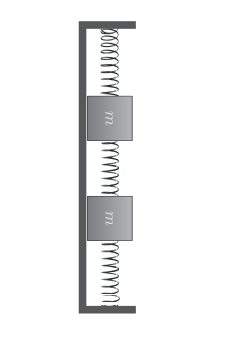
\includegraphics[width=0.2\textwidth]{three_springs_two_masses.png} \\ 
\end{center}

Equation (1) makes sense that $\frac{d^2u}{dt^2}$ is acceleration, making it essentially Newton's second law. Write equation (1) in detail:
$$
\begin{bmatrix}
m_1 & \\
    & m_2
\end{bmatrix}
\begin{bmatrix}
u_1'' \\
u_2''
\end{bmatrix}
+
\begin{bmatrix}
c_1+c_2 &-c_2\\
-c_2 & c_2+c_3
\end{bmatrix}
\begin{bmatrix}
u_1 \\
u_2
\end{bmatrix}
=0
$$
\\\\Part 2. Solve by eigenvectors

The solution for (1) is shaped like $u(t)=\sum_i a_i (\cos w^it) x^i + b_i (\sin w^it) x^i$, where $x^i$ is the $i$th constant vector. Inserting $u(t)$ in (1), we get $Kx=w^2Mx$, or better $M^{-1}Kx=w^2x$. You see that $x$ and $w^2$ are eigenvector and eigenvalue of $M^{-1}K$. And $M^{-1}$ can be calculated in a sudden since $M$ is a diagonal matrix. Now we only need $a_i$ and $b_i$ to get the complete solution, which can be done with the initial conditions.
\\\\Part 3. Solve by difference

Here we change the derivative $\frac{d^2u}{dt^2}$ with second order difference.

\section*{10 \& 11 Finite differences in time \& Least squares}
Part 1. Finite differences in time

For $\frac{du}{dt}=Au$, from 2.2 we have three methods to replace derivative with difference, which are equivalent to: 

Forward Euler $\frac{u_{n+1}-u_n}{\Delta t}=Au_n$

Backward Euler $\frac{u_{n+1}-u_n}{\Delta t}=Au_{n+1}$

Trapezoidal rule $\frac{u_{n+1}-u_n}{\Delta t}=\frac{1}{2}(Au_{n+1}+Au_n)$

For the Trapezoidal rule, it's equivalent to $u_{n+1}=(I-\frac{\Delta t}{2}A)^{-1}(I+\frac{\Delta t}{2}A)u_n$, where $G=(I-\frac{\Delta t}{2}A)^{-1}(I+\frac{\Delta t}{2}A)$ is the growth matrix, and $eig(G)=\frac{1+\frac{\Delta t}{2} eig(A)}{1-\frac{\Delta t}{2} eig(A)}$.
%=\frac{1+ \frac{\Delta t}{2}i}{1 - \frac{\Delta t}{2}i}$
\\\\ Part 2. Least squares (part1)

This is covered in 18.06 Linear Algebra.


\section*{12 Graphs and networks}
Part 1. Graph

As below, 4 nodes and 5 edges.  
\\\begin{center}
	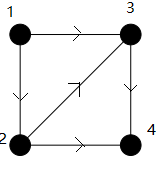
\includegraphics[width=0.2\textwidth]{four_nodes_five_edges.png} \\ 
\end{center}

We can use {\bfseries incidence} matrix $A$ to describe the graph, where each row stands for a edge, each column stands for a node, and -1 for start, 1 for end.
$$
A=
\begin{bmatrix}
-1 & 1 & 0 & 0 \\
-1 & 0 & 1 & 0 \\
0 & -1 & 1 & 0 \\
0 & -1 & 0 & 1 \\
0 & 0 & -1 & 1
\end{bmatrix}
$$

$A^TA$ equals to degree matrix subtracts adjacency matrix. Degree matrix $D$ is a diagonal matrix, where $D_{ii}$ is how many edges node $i$ connects. Adjacency matrix $W$ is a n($\#$nodes)*n matrix, where $W_{ij}= 1$ or 0 stands for there is/isn't an edge between node $i$ and $j$.
\\\\Part 2. Network

I will cover this part in the next section.


\section*{13 Kirchhoff's Current Law(KCL)}
\hspace*{0.5cm}The same graph in section 12. We can view each edge as an directed electric current. The {\bfseries Kirchhoff's Current Law} is that for every node, the sum of current is 0. For example, for node 3, $a+b+c=0$. The {\bfseries Kirchhoff's voltage Law} is that: the directed sum of the electrical potential differences (voltage) around any closed network is zero. 
\\\begin{center}
	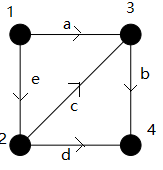
\includegraphics[width=0.2\textwidth]{four_nodes_five_edges_current.png}
\end{center}

KCL here in matrix form it's $A^Tw=0$ if there is no additional current source, where $w$ is current, $A$ is comes from section 12. $w=Ce$, where $C$ is constant, reciprocal of resistance, {\bfseries conductance}. If there is no battery on edges, $e=Au$, where $u$ is electric potential, otherwise $e=b-Au$, where $b$ is battery source. So finally we can write these equations in just one or two equations:

i. One equation: $A^TCAu=A^TCb-f$, called {\bfseries displacement method}. 

ii. Two equations: $C^{-1}w+Au=b$ and $A^Tw=f$,  called {\bfseries mixed method}.

\section*{14 Exam Review}

\section*{15 \& 16 Trusses and $A^TCA$}
A truss with 5 bars and 5 nodes(pins), every node have horizontal displacement $u^H$ and vertical displacement $u^V$. We have $Au=0$.


\section*{17 \& 18 Finite elements in 1D}
Part 1. The transpose of $A=d/dx$

For $A=d/dx$, $A^T=A^*=-d/dx$. A concrete proof will be given later. A rough proof is that:
$$
A=
\begin{bmatrix}
1 &  &  &  \\
-1 & 1 &  &  \\
 & -1 & 1 &  \\
 &  & -1 & 1
\end{bmatrix}
A^T=
\begin{bmatrix}
1 & -1 &  &  \\
 & 1 & -1 &  \\
&  & 1 & -1 \\
&  &  & 1
\end{bmatrix}
$$
Look at $A$ and $A^T$, from section 2, $A$ is first order (backward) difference, and $A^T$ is minus first order (forward) difference.
\\\\ Part 2. Inner product on functions \& concrete proof for $A^T=A^*=-d/dx$

For vectors, the inner product is defined as $a \cdot b=a^Tb=\sum_i a_ib_i$. For functions, the idea of inner product of functions comes from $\sum_i a_ib_i$ that $(e, w)=\int e(x)w(x)dx$. Functions are orthogonal when $(e, w)=0$.

$(Au)^Tw=u^T(A^Tw)$ holds for vectors, where $A=d/dx$. To generalize it to functions, $(Au)^Tw$ becomes $\int \frac{du}{dx}w(x)dx$, $u^T(A^Tw)$ becomes $\int u(x)(\frac{d}{dx})^Tw(x)dx$. We don't like the transpose sign in the integration, so use {\bfseries integration by parts} in calculus on $\int \frac{du}{dx}w(x)dx$: 
\begin{nscenter}
$\int \frac{du}{dx}w(x)dx=\int u(x)(-\frac{dw}{dx}dx)+ [u(x)w(x)]_{x=lower \, bound}^{x=higher \,  bound}$
\end{nscenter}
So when $[u(x)w(x)]_{x=lower \, bound}^{x=higher \,  bound} = 0$, you see the left side is $(Au)^Tw$, the right side is $u^T(A^Tw)$, where $A^T=-d/dx$! This is the concrete proof of $A^T=A^*=-d/dx$.
\\\\ Part 3. Weak form

The strong form of differential equation is $-\frac{d}{dx}(c\frac{du}{dx})=f(x)$. The weak form is multiplying (chosen, so known)test function $v(x)$ at both side, which does inner product:
\begin{nscenter}
	$\int c(x)\frac{du}{dx}\frac{dv}{dx} dx=\int f(x)v(x)dx$
\end{nscenter}
You may wonder where is the minus sign. The minus sign disappeared because $(d/dx)^T=-d/dx$ in inner product as discussed in part 1 and 2, or explicitly:
\begin{nscenter}
	$ \int f(x)v(x)dx = \int - \frac{d}{dx}(c\frac{du}{dx})v(x)dx = \int c(x) \frac{du}{dx}\frac{dv}{dx}dx - [c(x)\frac{du}{dx}v(x)]_{x=lower \, bound}^{x=higher \,  bound}$
\end{nscenter}

I think, the reason why we use test function here is that we can't deal with the strong form directly since there is $\frac{d}{dx}$ in $-\frac{d}{dx}(c\frac{du}{dx})=f(x)$.
\\\\Part 4. Galerkin's method

The {\bfseries Galerkin's method} is to discretize the weak form. First, substitute $u(x)$ in weak form with $U(x)=\sum_{1, 2, \cdots, n} U_i \phi _i(x)$, where $U_i$ is unknown number and $\phi _i(x)$ is chosen(so known) trail function. (I feel this substitution quite a bit likes variational inference.) Second, choose $n$ test functions $V_i$. For each $V_i$, inserting it to weak form, get 
\begin{nscenter}
	$\int c(x) (\sum_{j=1,\cdots, n} U_j\frac{d\phi_j}{dx})\frac{dV_i}{dx}=\int f(x)V_i(x)dx$
\end{nscenter}
For all $V_i$, we can write the equation above in matrix form that $KU=F$, where $K_{ij}=\int c(x)\frac{dV_i}{dx}\frac{d\phi_j}{dx}dx$, $U=[U_1, U_2, \cdots, U_n]^T$, $F_i=\int f(x)V_i(x)dx$. The finite element method(FEM) approximation is $\sum U_i\phi_i(x)$ for $u(x)$.

Frequently, test function $V_i$ is the same as trail function $\phi_i$, then $K_{ij} = K_{ji}$.
\\\\Part 5. Linear finite element

In linear finite element, the $\phi_i$, $U(x)=\sum U_i \phi_i(x)$ look like below
\\\begin{center}
	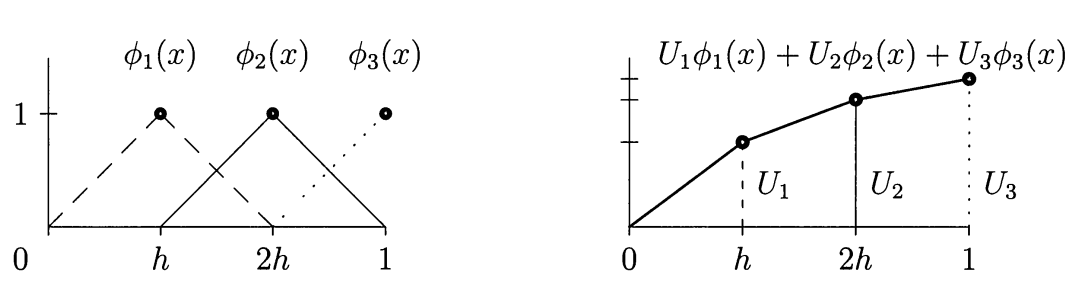
\includegraphics[width=0.9\textwidth]{linear_finite_element.png} \\ 
\end{center}

\section*{19 Quadratic/cubic elements}


\section*{23 \& 24 Laplace's equation}
Part 1. Laplace's equation and its solutions

Laplace's equation is {\bfseries $u_{xx}+u_{yy}=0$}. And magically, the solutions to this equation always come in pairs that $u(x, y)$ and $s(x,  y)$. The pairs come from $f(x+iy)$, where $u(x,y)=\Re[f(x+iy)]$ and $s(x,y)=\Im[f(x+iy)]$. 

Let's see some simple examples. Let $f(x+iy)=(x+iy)^n$, then the $(u(x,y), s(x,y))$ pair is  $(x, y), (x^2-y^2, 2xy), (x^3-3xy^2, 3x^2y-y^3), \cdots$.. You can check this is correct easily. A nice thing here is that if replace $x, y$ with $r\cos \theta, r\sin \theta$, which is in polar coordinate, the solutions can be nicely written as $u_n=r^n\cos n\theta, s_n=r^n\sin n\theta$, see part 4.

What I think the most magical thing for Laplace's equation is that $u(x,y)$ and $s(x, y)$ are perpendicular at the cross point! See explanation in part 3. For example, for $u(x,y)=x^2 - y^2$ and $s(x,y)=2xy$, let $s(x, y)=1$, then for $u(x,y)=1, 2, 3, \cdots$, there are many cross points of $u(x,y)$ and $s(x,y)$. At every cross point, $u(x,y)$ and $s(x, y)$ are perpendicular! It maybe hard to check this example with pencil and paper, but you can check $u(x,y)=x$ and $s(x,y)=y$ easily. What makes me think it magical is that because of the perpendicular, it acts as gradient descent! If we know the field of gradient($u(x,y)$), we don't need gradient descent anymore, we can get gradient's whole trace($s(x, y)$) at once!
\\\\Part 2. Analytic function and harmonic function

We know that any superposition of solutions to a linear equation(here Laplace's equation) is again a solution. For the example above, we have $f(x+iy)=f(z)=\sum_{n=0}^{\infty}c_nz^n$, called {\bfseries analytic function}, the solutions in pair are $u(x, y) = \Re[f(x+iy)]$ and $s(x, y) = \Im[f(x+iy)]$, called {\bfseries harmonic function}.
\\\\Part 3. The Cauchy-Riemann Equation

For $f(x+iy)$, we have $\frac{\partial^2 f(x+iy)}{\partial x \partial y}= \frac{\partial^2 f(x+iy)}{\partial y \partial x}$, resulting $\frac{\partial }{\partial y} f(x+iy)= 
i\frac{\partial }{\partial x} f(x+iy)$ because $\frac{\partial^2 f(x+iy)}{\partial x\partial y} = 
\frac{\partial }{\partial y} \frac{\partial f(x+iy)}{ \partial x} =
\frac{\partial }{\partial y}\frac{\partial f(x+iy)}{\partial z}\frac{\partial z}{\partial x}=
\frac{\partial }{\partial y}\frac{\partial f(x+iy)}{\partial z} $, and
$\frac{\partial^2 f(x+iy)}{\partial x\partial y} = 
\frac{\partial }{\partial x} \frac{\partial f(x+iy)}{ \partial y} =
\frac{\partial }{\partial x}\frac{\partial f(x+iy)}{\partial z}\frac{\partial z}{\partial y}=
\frac{\partial }{\partial x}\frac{\partial f(x+iy)}{\partial z}i $.

In part 1, we have $f(x+iy)=u(x, y) + is(x,y)$, and plug it here that $\frac{\partial }{\partial y}(u+is) = i\frac{\partial }{\partial x} (u+is)$. Match the real part and imaginary part, then we get the {\bfseries Cauchy-Riemann Equation}:
\begin{nscenter}
	$\frac{\partial u}{\partial x} = \frac{\partial s}{\partial y}$
	
	$\frac{\partial u}{\partial y} = -\frac{\partial s}{\partial x}$
\end{nscenter}
Why are $u(x,y)$ and $s(x, y)$ perpendicular at the cross point in part 1? Plugging the Cauchy-Riemann Equation in $u'(x,y) \cdot s'(x, y)$, which is the dot product of tangent line and equivalently the dot product of direction of $u'(x,y)$ and $s'(x, y)$, $u'(x,y) \cdot s'(x, y) = (\frac{\partial u}{\partial x}, \frac{\partial u}{\partial y}) \cdot (\frac{\partial s}{\partial x}, \frac{\partial s}{\partial y}) =  
(\frac{\partial u}{\partial x}, \frac{\partial u}{\partial y}) \cdot (-\frac{\partial u}{\partial y}, \frac{\partial u}{\partial x}) = 0$.
\\\\ Part 4. Polar coordinate: Laplace's equation in a circle

In part1, we said, if we replace $x, y$ with $r\cos \theta, r\sin \theta$, which is in polar coordinate, the solutions can be nicely written as $u_n=r^n\cos n\theta, s_n=r^n\sin n\theta$. Why?

First, $x+iy=r\cos \theta +i r\sin \theta=r(\cos \theta +i\sin \theta)=re^{i\theta}$.

Then, $(re^{i\theta})^n=re^{in\theta}=r^n(\cos n\theta + i \sin n\theta)=r^n \cos n\theta + i r^n \sin n\theta$.

Finally, $u(x, y)$, $s(x, y)$ are the real and imaginary part that $r^n\cos n\theta, r^n\sin n\theta$.

\section*{25 \& 26 Fast Poisson solvers}
Part 1. $K$ in 2D

For {\bfseries Poisson's equation} $-u_{xx}-u_{yy}=f(x, y)$, we can discretize the derivative with second difference and describe it as $KU=F$. We have seen $KU=F$ in 1-dimension in section 17 \& 18. Let's discretize it in a 2-dimension square. 

First, discretize the 2D square as meshes with meshwidth $h$, as below. The Poisson's equation for a molecule centered at position $(i, j)$ (the molecules at the boundary are not take into account) is as below, looks like a filter, aha?
\begin{nscenter}
$4U_{i,j} - U_{i, j-1} - U_{i-1, j} - U_{i+1, j}- U_{i, j+1}=h^2f(ih, jh)$
\end{nscenter}
For molecules next to the boundary, the corresponding $U$ is dropped, or concretely, moved to the right side of the equation according to the book. 

So we know the corresponding row in $K$ for every molecule. For example, if give the index from left to right and bottom to top, the corresponding(6-th) row in $K$ for $(1, 2)$ is $[-1, 0, 0, 0, 0, 4, -1, 0 ,0, 0, -1, \cdots]$ with length of $5^2$.
\\\begin{center}
	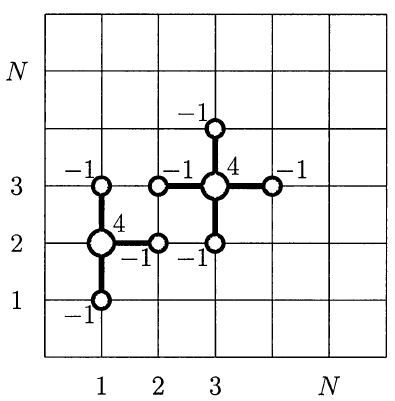
\includegraphics[width=0.3\textwidth]{Poisson_mesh.png}
\end{center}
Part 2. $K$ in 2D with Kronecker product

There exists a way to generate $K$ in 2D with math, {\bfseries Kronecker product}. The Kronecker product is defined as:
\begin{nscenter}
	$\mathbf{A}\otimes\mathbf{B} = \begin{bmatrix} a_{11} \mathbf{B} & \cdots & a_{1n}\mathbf{B} \\ \vdots & \ddots & \vdots \\ a_{m1} \mathbf{B} & \cdots & a_{mn} \mathbf{B} \end{bmatrix}$
\end{nscenter}

We know the $K$ in 1D should be 
$$
K_{1D}=
\begin{bmatrix}
2 & -1 &  &  \\
-1 & 2 & -1 &  \\
&  \cdot & \cdot & \cdot \\
&  & -1 & 2
\end{bmatrix}
$$

Then $K$ in 2D is 
$$
K=kron(I, K_{1D}) + kron(K_{1D},I)=
\begin{bmatrix}
K_{1D}+2I & -I &  &  \\
-I & K_{1D}+2I & -I &  \\
&  \cdot & \cdot & \cdot \\
&  & -I & K_{1D}+ 2I
\end{bmatrix}
$$
\\ Part 3. Solve Poisson's equation with (elimination and fill-in) or cyclic odd-even reduction

A simple to solve Poisson's equation is elimination. This is straightforward but time-consuming comparing to other good ideas.

If we change the index of these molecules as counting every 2 molecules, we can do elimination faster, because $K$ would be more organized inside. For example, for 3*3 molecules, from left to right and bottom to top, we assign the index as 
\\\begin{nscenter}
	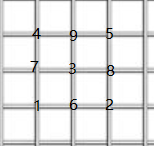
\includegraphics[width=0.3\textwidth]{cyclic_odd-even_reduction.png}
\end{nscenter}
\\\\ Part 3. Solve Poisson's equation in 1D with eigenvectors

For $K$ in 1D, it's very special that second order difference, which enables us to find its eigenvectors($y_i$) and eigenvalues($\lambda_i$) easily even with pencil and paper.
From 18.06, if $A$ is invertible, $A$ and $A^{-1}$ have the same eigenvectors, and the eigenvalues are reciprocal of each other. So we know the eigenvectors and eigenvalues for $K^{-1}$. So for $Ku=f$, $u=K^{-1}f$. Recall the meaning of eigenvectors in 18.06, we decompose $f$ to eigenvectors' direction as $f=\sum a_iy_i$, then $u=K^{-1}f=\sum \frac{1}{\lambda_i}a_iy_i$, or $u=S\Lambda^{-1}S^{-1}f$ in matrix form where $S, \Lambda$ are eigenvector and eigenvalue matrix.

For $K$ in 2D, the solution comes from the same idea, but we need help of the Discrete Sine Transform in part 4.
\\\\Part 4. The Discrete Sine Transform in 1D

In 1D, column $k$ of the eigenvector matrix $S$ contains the eigenvector $y_k$. The number $S_{jk}=\sin \frac{jk\pi}{N+1}$ is the $j$th component of that eigenvector. For our example in part 1 with $N +1$ = 6, $\frac{jk\pi}{N+1}$ is always multiple of $\frac{\pi}{6}$. ($\sin \frac{1\pi}{6}, \sin \frac{2\pi}{6}, \sin \frac{3\pi}{6}, \cdots$) is a list that ($\frac{1}{2}, \frac{\sqrt{3}}{2}, 1, \frac{\sqrt{3}}{2}, \frac{1}{2}, 0, -\frac{1}{2}, -\frac{\sqrt{3}}{2}, -1, -\frac{\sqrt{3}}{2}, -\frac{1}{2}, -0, \cdots$(repeat forever)).
The $k$th column of $S$($k$th eigenvector $y_k$) just takes every $k$th number from that list. So for our example, here are the first five eigenvectors:
\\\begin{nscenter}
	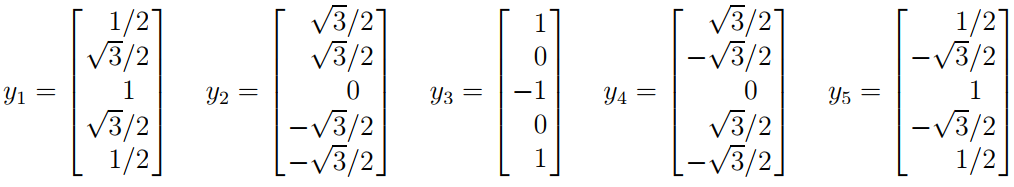
\includegraphics[width=1\textwidth]{discrete_sine_transform_eigenvectors.png} \\ 
\end{nscenter}

Those eigenvectors are orthogonal ! This is guaranteed by the symmetry of $K$. All
these eigenvectors have length 3, so $S/\sqrt{3}$ is an orthonormal matrix $Q$, with $Q^TQ = I$. What's more, for this very special example, $S$ and $Q$ are also symmetric, so $Q^{-1}=Q^T=Q$.
\\\\ Part 5. Solve Poisson's equation in 2D with eigenvectors

To extend this eigenvalue(Discrete Sine Transform) method to two dimensions, we need the eigenvalues and eigenvectors of K in 2D. The key point is that the $N^2$ eigenvectors of $K$ in 2D are separable that each eigenvector $y_{kl}$ separates into a product of sines, where $(i ,j)$ is for $F_{ij}$ and $U_{ij}$ in Poisson's equation:
%maybe wrong (I think $kl$ in $y_{kl}$ means $k$ multiply $l$)
\begin{nscenter}
	the $(i, j)$ component of $y_{kl}$ is $\sin \frac{ik\pi}{N+1} \sin \frac{jl\pi}{N+1}$
\end{nscenter}
The eigenvalue in two dimensions is the sum $\lambda_k + \lambda_l$ of one-dimensional eigenvalues:
\begin{nscenter}
	 $\lambda_{kl}=(2-2\cos \frac{k\pi}{N+1}) + (2- 2\cos \frac{l\pi}{N+1})$
\end{nscenter}

Now the solution of $KU = F$ in 2D comes by a two-dimensional sine transform:
\begin{nscenter}
	$F_{ij}=\sum\sum a_{kl} \sin \frac{ik\pi}{N+1} \sin \frac{jl\pi}{N+1}$, $U_{ij}=\sum\sum \frac{a_{kl}}{\lambda_{kl}} \sin \frac{ik\pi}{N+1} \sin \frac{jl\pi}{N+1}$
\end{nscenter}

Or extremely in matrix form that for $KU=F$, $U=K^{-1}F=S\Lambda^{-1}S^{-1}F$ because $K=S\Lambda S^{-1} \Leftrightarrow K^{-1} = S\Lambda^{-1}S^{-1}$, which comes from 18.06 that if $A$ is invertible, $A$ and $A^{-1}$ have the same eigenvectors, and the eigenvalues are reciprocal of each other.


\section*{28 \& 29 Fourier series}
Part 1. Fourier sine/cosine series

{\bfseries Fourier sine series}: 
\begin{nscenter}
	$S(x)=b_1\sin x + b_2\sin 2x + b_3 \sin3x + \cdots=\sum_{n=1}^{\infty}b_n \sin nx$
\end{nscenter}
The item $\sin 0x$ is dropped off since it equals to 0, but not for Fourier cosine series. To get the coefficient $b_i$,  first recall orthogonality of these sines that:
\begin{nscenter}
	$\int_0^{\pi} \sin nx \sin kx dx = 0$ if $n\neq k$ \qquad (1)
\end{nscenter}
Then we take advantage of that orthogonality that multiply $\sin kx$ on both sides of Fourier sine series, and take integral:
\begin{nscenter}
	$\int_0^{\pi} S(x) \sin kx dx = \int_0^{\pi} b_1 \sin x \sin kx dx + \cdots + \int_0^{\pi} b_k \sin kx \sin kx dx + \cdots$
\end{nscenter}
Because of orthogonality above, all items in the right side is 0 except \\$\int_0^{\pi} b_k \sin kx \sin kx dx$, which is $\frac{\pi}{2}$. So:
\begin{nscenter}
	$b_k = \frac{2}{\pi} \int_0^{\pi} S(x) \sin kx dx = \frac{1}{\pi} \int_{-\pi}^{\pi} S(x) \sin kx dx$
\end{nscenter}
, where the last equal sign comes from $S(x)=-S(x)$.

Fourier cosine series is similar to Fourier sine series $C(x)$.
\\\\Part 2. Fourier Complete series and Fourier Complex Exponential Series

$S(x) + C(x)$ gives the {\bfseries Fourier Complete Series}:
\begin{nscenter}
	$F(x)=a_0 + \sum_{n=1}^{\infty}a_n \cos nx + \sum_{n=1}^{\infty}b_n \sin nx$
\end{nscenter}
The coefficients can be solved similar to Fourier sine series as:
\begin{nscenter}
	$a_0 = \frac{1}{2\pi} \int_{-\pi}^{\pi} F(x) dx$ \\
	$a_k = \frac{1}{\pi} \int_{-\pi}^{\pi} F(x) \cos kx dx$ \\
	$b_k = \frac{1}{\pi} \int_{-\pi}^{\pi} F(x) \sin kx dx$
\end{nscenter}
The integral range $[-\pi, \pi]$ comes from that to utilize the orthogonality as equation (1), the range need to be $[-\pi, \pi]$.

{\bfseries Fourier Complex Exponential Series} is:
\begin{nscenter}
	$F(x)=c_0 + c_1 e^{ix} + c_{-1} e^{ix} + \cdots + \cdots = \sum_{n=-\infty}^{\infty}c_n e^{inx}$, where $i^2=1$
\end{nscenter}
The coefficients are given as:
\begin{nscenter}
$c_n = \frac{1}{2\pi} \int_{-\pi}^{\pi} F(x) e^{-inx} dx$
\end{nscenter}
\\\\ Part 3.  Application: Laplace's Equation in a circle

For Laplace's Equation in a circle, combination of all solutions is:
\begin{nscenter}
	$u(r, \theta) = a_0 + a_1r\cos\theta + b_1r\sin\theta + a_2r^2\cos2\theta + b_2r^2\sin2\theta+\cdots$ (2)
\end{nscenter}
For example, we let $r=1$. The coefficients are automatically solved since equation (2) is exactly the Fourier Complete series, in which we can get coefficients easily.



\section*{30 \& 31.a Discrete Fourier series \& fast Fourier transform(FFT)}
Part 1. The Discrete Fourier Transform

Discretize Fourier Complex Exponential Series $F(x)=\sum_{k=-\infty}^{\infty}c_k e^{ikx}$ to $f_j=\sum_{k=0}^{N-1}c_kw^{jk}$, where $w$ is $N$th sqrt root of 1($w^N=1$), or in matrix form $f=F_Nc$. The solution of coefficients is discreted to $c_k=\frac{1}{N}\sum_{j=0}^{N-1}f_j\bar w ^{jk}$, or in matrix form $c=F^{-1}_Nf$. From the Fourier matrix below, you can see the first row is all 1 element, so $c_0$ is always $(\sum f_i) / N$.

The Fourier matrix is 
$$
F_N =
\begin{bmatrix}
1 & 1 & 1 & \cdots & 1\\
1 & w & w^2 & \cdots & w^{n-1}\\
1 & w^2 & w^4 & \cdots & w^{2(n-1)}\\
\vdots &\vdots&  \vdots & \ddots &  \vdots \\
1 & w^{n-1} & w^{2(n-1)} & \cdots & w^{(n-1)^2}
\end{bmatrix}
$$
where $(F_N)_{ij}=w^{ij}$, indexes of $i, j$ start from 0, since we are in EE area now:)

The Fourier matrix is orthogonal. To check this, note that because we are in complex area now, you show do $a^*b(\bar a^Tb)$ instead of $a^Tb$. And $\hat {F_N}=\frac{1}{\sqrt N}F_N$ is orthonormal. So $F_N^{-1}=\frac{1}{N}F^*$.
\\\\Part 2. FFT

A FFT algorithm is a method to compute the discrete Fourier transform of a sequence, or its inverse, in which the {\bfseries Cooley–Tukey algorithm} is a famous one. And that's already given in MIT 18.06 section 26 part 3.

\section*{31.b \& 32.a Convolution}
Part 1.  Convolution and Fourier coefficients

There is a way to introduce convolution from Fourier series. When two Fourier complex series $f(x) = \sum c_k e^{ikx}$ and $g(x) = \sum d_k e^{ikx}$ multiply, what's the Fourier coefficients of the product $f(x)g(x)$? The coefficients come from convolving the vector of $c$'s and the vector of $d$'s, denoted as $c * d$. The coefficients are not $c \odot d$ because when we combine these two Fourier series to just one Fourier series $f(x)g(x) = \sum a_k e^{ikx}$, the $a_k e^{ikx}$ comes from $c_k e^{ik'x}$ and $d_k e^{ik''x}$, where $k = k' + k''$. You know for $k = k' + k''$, there are a lot of combinations. Once you figure out these combinations in formula form, you get the detail(expansion) of $c * d$. The other magical thing is that though $c \odot d$ is not the correct coefficient, it($2\pi c \odot d$) is the correct coefficient of $f(x) * g(x)$ with a factor $2\pi$.

The $n$th component of $c*d$ is $\sum_{k=-\infty}^{\infty}c_kd_{n-k}$. This is easy to understand that $k + (n-k)=n$, where we get the all the possible combinations of $n$.

My understand: Suppose $x$ is an image, $s$ is a filter(e.g, sobel), $x*s$ means that $x$ are (Fourier)coefficient of $X$ and $s$ are coefficient of $S$, $x*s$ is the coefficient of $X\cdot S$. We never see $X, S$ and $X\cdot S$ above though we got $x*s$.
\\\\ Part 2. Cyclic convolution, convolution and multiplication 

Suppose $f(w)=1+2w+4w^2$, $g(w)=3+5w$ and $w^3=1$, so we have {\bfseries cyclic convolution} with $N=3$. To write $f(w)g(w)$ in $w$, a way we have known is $(1+2w+4w^2)(3+5w)=13+ 26w+27w^2$. The second way, which I think is essentially same as the first way, only deal with the coefficients, is that $c \circledast d = (1, 2, 4) \circledast (3, 0 ,5) = (13, 26, 17)$, where $\circledast$ means cyclic convolution. You can understand the calculation that firstly, the result must be length of 3 because $w^3=1$, secondly the 0th result element comes from (0th, 0th), (1th, 2th) and (2th, 1th) input because $w^3=1$, the rest result elements come from the same way. 

If we do non-cyclic convolution that $c*d$, the result is $(3, 6, 17, 10, 20)$. The  result length is sum of length $c, d$ minus 1, which is not a coincidence, because for $w^0, w^1, w^2$ and $w^0, w^1, w^2$, of course we get $w^0, w^1, w^2, w^3, w^4$. The connection with multiplication is that $(3, 6, 17, 10, 20) \cdot (10^0, 10^1, 10^2, 10^3, 10^4)=421*503$.
\\\\ Part 3. Cyclic convolution rules
\\\\ Part 4. Convolution by matrices 

\section*{32.b \& 33.a Filters}
Filtering (the key step in signal and image processing) is a convolution. For example, a lowpass filter that (second order average) $y_n=\frac{1}{4}x_{n-1} + \frac{2}{4}x_n + \frac{1}{4}x_{n+1}$, and a highpass filter that $D=K/4$, where $K$ is the second order difference matrix. The convolution $y = a * x$ can be written in matrix form $y=Ax$. For example, the lowpass filter can be written as 
$$
\begin{bmatrix}
\cdot \\
y_0 \\
y_1 \\
y_2 \\
\cdot
\end{bmatrix}
=
\frac{1}{4}
\begin{bmatrix}
\cdot & \cdot \\
1 & 2 & 1 \\
 & 1 & 2 & 1 \\
 &   & 1 & 2 & \cdot \\
 &   &   & \cdot & \cdot 
\end{bmatrix}
\begin{bmatrix}
x_{-1} \\
x_0 \\
x_1 \\
x_2 \\
\cdot
\end{bmatrix}
= Ax 
= a* x
$$
For this lowpass filter, you see that for the input $x_{low}=(., 1, 1, 1, 1, .)$, the output $y$ is the same as input $x$. But for the input $x_{high}=(., 1, -1, 1, -1, .)$, the output $y$ is $(0, 0, 0, 0)$. The low/high in lowpass/highpass means  frequency $\omega$ in $e^{\omega x + \phi}$.

Except allowing the low frequency component, the lowpass filter also remove the noise from the signal, since random noise tends to be high frequency. But filter also blurs significant detail in the input $x$. The big problem of signal processing is to choose the best filter.

In fact, we have a better way that frequency response to analyze all frequencies. For the lowpass filter, the frequency response is 
\begin{nscenter}
	$A(\omega)=A(e^{i\omega})=\frac{1}{4}e^{-i\omega} + \frac{2}{4} + \frac{1}{4}e^{iw} = \frac{1}{2}(1+\cos \omega)$
\end{nscenter}
So we just insert different frequency to this equation to get corresponding response. For example, $A(0)=1, A(\pi)=0$, which means low pass. All frequency responses are given as below:
\\\begin{nscenter}
	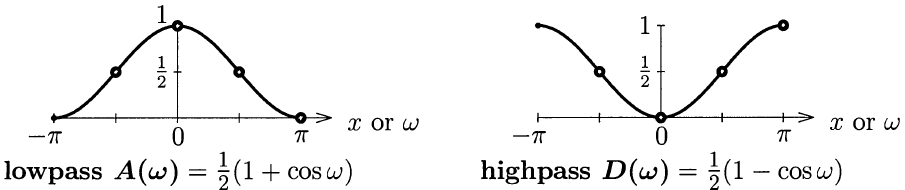
\includegraphics[width=0.8\textwidth]{lowpass_and_highpass.png} \\ 
\end{nscenter}

\section*{33.b \& 34 Fourier Integrals}
A Fourier series is perfect for a $2\pi$-periodic function. The only frequencies in $\sum c_ke^{ikx}$ are whole numbers $k$. When $f(x)$ is not periodic, all frequencies $k$ are allowed. That sum has to be replaced by an integral $\int_{-\infty }^{\infty}\hat f (k) e^{ikx} dk$. Because the symbol of coefficients $c_k$ changed to $\hat f(k)$, we use the new symbol to get:

i. Transform $f(x)$ to $\hat f(k)$: $\hat f(k)=\int_{-\infty }^{\infty} f (x) e^{-ikx} dx$, which can be get by analogy of $c_k = \frac{1}{2\pi}\int_{-\pi}^{\pi}f(x)e^{-ikx}dx$.

ii. Reconstruction $\hat f (k)$ to $f(x)$: $f(x)=\frac{1}{2\pi}\int_{-\infty }^{\infty}\hat f (k) e^{ikx} dk$, which can be get by analogy of $f(x)=\sum_{k=-\infty}^{\infty}c_ke^{-ikx}$.

\section*{35 Deconvolution}
If we know $G, B$ in $G * U = B$, how to get $U$? This can be done with the idea in part 1 of section 31.b \& 32.a Convolution  that $G *U=B \Rightarrow \hat G \hat U = \hat B \Rightarrow \hat U = \hat B / \hat G$, where hat means that $\hat F = \sum Fe^{ikx}$.

%\\\begin{center}
%	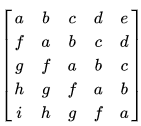
\includegraphics[width=0.2\textwidth]{Toeplitz_matrix1.png} \\ 
%\end{center}


\section{Things to do}
Pay attention to variational inference and Fourier transform(KCF )!

Function is mapping. Map set $x$ to $y$, and $f$ (in $f(x)$) is the rule to map!

Functional Analysis

Appro the CNN with a function which can be solved in a sudden. For example, for Lenet, the network is mapping a two-dimension matrix a vector with length 10(0~9). If there exist some basic mapping functions, we can take combinations of them(as f), then approximate the Lenet with f. The approximation process could be easy, we can just compare the output vector, define a loss, then use SGD.

PS1: This method may work if we PS2: This idea should be bad because the kernel is essentially extract appearance feature, and the $(Objs_i)^T(Objs_{i+1})$ is just doing a very simple classification. If we can find a kernel to extract features as cyclic, which don't need to fill the whole cyclic matrix, we can fill the other vectors in the cyclic matrix, for the objects $Objs_i$ in frame $i$ and similar $Objs_{i+1}$, we can just do the association by $(Objs_i)^T(Objs_{i+1})$, which measures the similarity among all objects in frame $i$ and all objects in frame $j$.
\end{spacing}
\end{document}